\chapter{Hypergraphe-Percol' : la généralisation du Single-Linkage dans l'espace euclidien} 
\label{chap:hgp_clusterer}
\rouge{15 avril - 20 avril}


Nous avons vu que le Robust Single-Linkage \cite{RobustSingleLinkage2010} ou (H)DBSCAN \cite{HDBSCAN, HDBSCAN2017} imposent à un n\oe ud d'avoir $K$ voisins  (ou au moins d'être à la frontière de l'un de ces $K$-cœurs) pour apparaître au sein d'un cluster. Dans le même temps, une simple arête suffit pour connecter deux n\oe uds.

C'est cette asymétrie entre les contraintes (fortes) imposées aux points et celles (lâches) vis-à-vis des arêtes que nous allons réparer dans le présent chapitre.

Des contraintes plus fortes (d'ordre supérieur) imposées aux liens peuvent être encodées en recourant aux hypergraphes, et plus particulièrement aux complexes simpliciaux.
La réparation naturelle consiste à renforcer aussi la notion de connexion. 

Le bon objet à construire n'est plus le graphe géométrique, mais le complexe de \v Cech \cite{Cech1932, BobrowskiKahle} ; et la bonne notion de composante connexe n'est plus une composante de sommets reliés par des arêtes, mais une composante de $(K-1)$-simplexes reliés par des interactions d'ordre supérieur (ce que nous avons appelé des $K$-polyèdres).

Nous ne chercherons pas ici à forcer une partition à chaque niveau. Pour $K\ge 2$, les amas discrets de forte densité (\Def~\ref{def:HDC_discret}) peuvent se recouvrir (\emph{cf}. l'exemple du chapitre précédent) ; la généralisation correcte du Single-Linkage doit donc produire, elle aussi, une hiérarchie de recouvrements.

À l'instar de la définition du Single-Linkage (\emph{via} l'analyse persistante de graphes géométriques, \emph{cf}. \Def~\ref{def:dendrogramme_gg}), la généralisation du Single-Linkage, que nous avons baptisée HGP-Clusterer (\Def~\ref{def:hgp_clusterer}), est pour l'instant toute théorique. Nous verrons au cours des chapitres suivants (dédiés à la généralisation et à la construction de l'arbre minimum couvrant) comment extraire cette hiérarchie en pratique.

\Contributions{Les résultats présentés ici reprennent et reformulent \cite{BibiAppliedNetworkScience}. La reformulation adoptée dans ce manuscrit, plus naturelle et plus simple, a été permise grâce à notre définition d'un amas de forte densité $K$-NN \emph{discret} (\Def~\ref{def:HDC_discret}). Le résultat principal de ce chapitre (\Th~\ref{th:cech_kpolyedres_knn}) découle alors simplement de la construction d'un graphe d'intersection sur ce que nous avons appelé les régions témoins d'une forte densité.}

\section{Du graphe géométrique au complexe de \v Cech : les $K$-polyèdres}

Le point de vue sur le Single-Linkage développé dans la partie~I que nous reprenons comme point de départ est celui d'une analyse persistante sur des graphes géométriques (\Def~\ref{def:dendrogramme_gg}). La généralisation naturelle consiste à remplacer les graphes par des hypergraphes\footnote{Un graphe est la donnée d'un ensemble de sommets noté $V$ (pour \emph{vertices} en anglais) et d'un ensemble de relation binaires entre ces sommets, les arêtes $E$ (\emph{edges} en anglais). Dans le cas d'un \emph{hyper}graphe, les arêtes deviennent des hyper-arêtes, c'est-à-dire qu'elles ne sont plus nécessairement binaires mais peuvent encoder des relation d'ordre supérieur : des triangles, des tétraèdres, \emph{etc}.}.
Plus précisément, une sous-famille des hypergraphes va nous servir au cours de ce manuscrit : les complexes simpliciaux \cite{Munkres}. Un complexe simplicial est un hypergraphe pour lequel la présence d'une hyper-arête entraîne la présence de toutes les sous-hyper-arêtes. Par exemple, la présence d'un tétraèdre entraîne la présence de ses quatre ``facettes'' (triangles), de ses quatre arêtes (et bien-sûr des quatre sommets, que l'on peut voir comme des hyper-arêtes d'ordre $0$).

Il devient alors possible de remplacer les composantes connexes ordinaires par une ``connectivité'' d'ordre supérieur.

\subsection{Le complexe de \v Cech}

\begin{Definition}{Complexe de \v Cech \cite{Cech1932, Munkres, BoissonnatChazalYvinec}}{cech_complexe}
Soit $\X\subset \mathbb R^p$ un nuage fini et $r\ge 0$. Le \emph{complexe de \v Cech} de rayon $r$ est le complexe simplicial
\[
    \check C(\X,r) \eqdef \left\{\sigma\subseteq \X \ \middle|\  \bigcap_{x\in \sigma}\overline B(x,r)\neq \varnothing \right\}.
\]
Autrement dit, un ensemble fini $\sigma\subseteq \X$ est un simplexe de $\check C(\X,r)$ si et seulement s'il existe un point $y\in\mathbb R^p$ situé à distance au plus $r$ de tous les sommets de $\sigma$.
\end{Definition}

\textcolor{red}{Parler aussi des complexes de Vietoris--Rips ? notamment pour les approximations dans le cas de figure non euclidien ? Ou bien y consacrer un court chapitre ? }

\Remarque{Le $1$-squelette de $\check C(\X,r)$ n'est autre que le graphe géométrique $\mathcal G(\X,r)$ introduit au \S~\ref{chap:single-linkage_trois_vues} : une arête $\{x,x'\}$ apparaît exactement lorsque $\overline B(x,r)\cap \overline B(x',r)\neq\varnothing$, c'est-à-dire lorsque $\norme{x-x'}\le 2r$.}

Plus généralement, un $K$-simplex de $\check C(\X,r)$ encode une interaction entre $K+1$ points qui peuvent être simultanément vus depuis une même boule de rayon $r$. C'est précisément ce type d'information (indiquant la densité locale) qui manque au Single-Linkage classique et qui est la source de l'effet de chaînage.

\subsection{Les $K$-polyèdres}

\begin{Definition}{Graphe des $(K-1)$-simplexes et $K$-polyèdres}{k_polyedres}
Soit $K\in \IntervalleEntiers{1,|\X|}$ et $r\ge 0$. On note $\check C_{K-1}(\X,r)$ l'ensemble des simplexes de dimension $K-1$ du complexe de \v Cech.

On leur associe le graphe
\[
    \Gamma_K(\X,r)
\]
dont les sommets sont les éléments de $\check C_{K-1}(\X,r)$, deux sommets $\sigma$ et $\tau$ étant reliés dès que $\sigma\cup\tau$ est encore un simplex de $\check C(\X,r)$.

Un \emph{$K$-polyèdre} de $\check C(\X,r)$ est alors l'ensemble des points de $\X$ apparaissant dans une composante connexe de $\Gamma_K(\X,r)$.
\end{Definition}

\Remarque{Cette définition prolonge exactement la notion usuelle de composante connexe. Pour $K=1$, les sommets de $\Gamma_1(\X,r)$ sont les points de $\X$ et ses arêtes sont celles du graphe géométrique ; les $1$-polyèdres sont donc les composantes connexes ordinaires. Pour $K=2$, les sommets de $\Gamma_2(\X,r)$ sont les arêtes de $\check C(\X,r)$ et deux arêtes partageant un sommet deviennent adjacentes dès que le triangle qu'elles forment apparaît.
\textcolor{red}{Illustrer ? ou est-ce déjà assez clair ?}
Cette façon de connecter entre eux des simplexes (vu comme des cliques sur sur un graphe) au moyen d'une clique plus grande est appelée \emph{clique percolation} \cite{KCliquePercolation}. Pour le cas plus général des complexes simpliciaux, \textsc{Atkin} avait déjà défini en 1972 ce qu'il nommait la $q$-\emph{connectivity} \cite{Atkin1972}. Aujourd'hui, l'usage serait plutôt d'employer le terme \emph{(up) face percolation} \cite{HirschValesin2025}.}

%\Remarque{L'on peut, de façon équivalente, ne tester l'adjacence qu'au moyen des seuls $K$-simplexes. Si $\sigma\cup\tau$ possède strictement plus de $K+1$ sommets, on relie encore $\sigma$ à $\tau$ en remplaçant les sommets un par un. Le graphe obtenu n'est autre qu'un graphe de Johnson, donc il est connexe.}

\begin{Definition}{HGP-Clusterer (HGP pour Hypergraphe-Percol')}{hgp_clusterer}
Pour $K\in \IntervalleEntiers{1,|\X|}$, on définit \emph{Hypergraphe-Percol'} (acronyme : HGP) par
\[
    \theta^{\mathrm{HGP}}_K(r) \eqdef \left\{\text{$K$-polyèdres de } \check C(\X,r)\right\},
    \qquad r\ge 0.
\]
Autrement dit, HGP-Clusterer observe l'évolution des $K$-polyèdres au fil de la filtration du complexe de \v Cech.
\end{Definition}

\Remarque{La filtration $r\mapsto \check C(\X,r)$ est croissante, donc le graphe $\Gamma_K(\X,r)$ l'est aussi. Les $K$-polyèdres ne peuvent ainsi que croître et fusionner lorsque $r$ augmente. Pour $K=1$, on retrouve exactement le Single-Linkage de la partie~I.}

\begin{figure}[!ht]
    \centering
    \begin{subfigure}[b]{0.48\textwidth}
        \centering
        \begin{tikzpicture}[scale=0.55]
            \def\r{1.5}
            \pgfmathsetmacro{\rprime}{2*sqrt(3)/3*\r}
            \pgfmathsetmacro{\h}{\r*sqrt(3)}

            \coordinate (C) at (-\r, 0);
            \coordinate (D) at (\r, 0);
            \coordinate (A) at (-\r-\h, \r);
            \coordinate (B) at (-\r-\h, -\r);
            \coordinate (E) at (\r+\h, \r);
            \coordinate (F) at (\r+\h, -\r);

            \begin{scope}[on background layer]
                \fill[blue!18] (A) -- (B) -- (C) -- cycle;
                \fill[red!18]  (D) -- (E) -- (F) -- cycle;
            \end{scope}

            \templateNuage[\r]

            \foreach \P in {A,B,C,D,E,F} {
                \draw[dashed, gray!70] (\P) circle (\rprime);
            }

            \node[blue!70!black] at (-4.2,2.6) {$ABC$};
            \node[red!70!black]  at (4.2,2.6) {$DEF$};
            \node[above=4pt] at ($(C)!0.5!(D)$) {$CD$};
        \end{tikzpicture}
        \caption{Complexe de \v Cech pour $K=2$}
        \label{fig:chap2_cech_exemple}
    \end{subfigure}
    \hfill
    \begin{subfigure}[b]{0.48\textwidth}
        \centering
        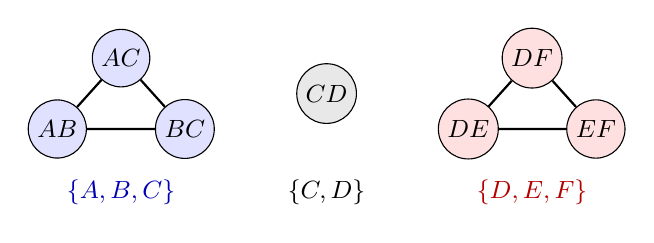
\begin{tikzpicture}[scale=0.9, every node/.style={font=\small}]
            \node[circle, draw, fill=blue!12, inner sep=2pt] (ab) at (0,1.0) {$AB$};
            \node[circle, draw, fill=blue!12, inner sep=2pt] (ac) at (0.9,2.0) {$AC$};
            \node[circle, draw, fill=blue!12, inner sep=2pt] (bc) at (1.8,1.0) {$BC$};
            \draw[thick] (ab)--(ac)--(bc)--(ab);

            \node[circle, draw, fill=gray!18, inner sep=2pt] (cd) at (3.8,1.5) {$CD$};

            \node[circle, draw, fill=red!12, inner sep=2pt] (de) at (5.8,1.0) {$DE$};
            \node[circle, draw, fill=red!12, inner sep=2pt] (df) at (6.7,2.0) {$DF$};
            \node[circle, draw, fill=red!12, inner sep=2pt] (ef) at (7.6,1.0) {$EF$};
            \draw[thick] (de)--(df)--(ef)--(de);

            \node[blue!70!black] at (0.9,0.1) {$\{A,B,C\}$};
            \node at (3.8,0.1) {$\{C,D\}$};
            \node[red!70!black] at (6.7,0.1) {$\{D,E,F\}$};
        \end{tikzpicture}
        \caption{Le graphe $\Gamma_2(\X,r)$ associé}
        \label{fig:chap2_gamma2_exemple}
    \end{subfigure}
    \caption{Exemple de $2$-polyèdres sur la configuration à six points du chapitre précédent. Au rayon $r'=\frac{2\sqrt 3}{3}r$, le complexe de \v Cech contient deux triangles $ABC$ et $DEF$ ainsi que l'arête $CD$. Les composantes connexes du graphe $\Gamma_2(\X,r')$ donnent alors trois $2$-polyèdres, à savoir $\{A,B,C\}$, $\{C,D\}$ et $\{D,E,F\}$. On voit déjà apparaître le phénomène essentiel : pour $K\ge 2$, les polyèdres peuvent se recouvrir.}
    \label{fig:chap2_exemple_kpolyedres}
\end{figure}

La \Fig~\ref{fig:chap2_exemple_kpolyedres} illustre la différence de nature entre la connexité ordinaire et la connexité d'ordre supérieur. Dans le cas $K=2$, ce ne sont plus les points qui percolent directement, mais les arêtes, recollées entre elles par des triangles.

\section{$K$-polyèdres de \v Cech et amas discrets de forte densité $K$-NN}

La première partie a introduit l'estimateur $K$-NN de densité des $K$ plus proches voisins (\Def~\ref{def:K-NN}) et les amas \emph{discrets} de forte densité qui lui sont associés (\Def~\ref{def:HDC_discret}). Rappelons qu'à rayon $r>0$ fixé, le niveau supérieur s'écrit
\[
    L_K(r) \eqdef \left\{ y\in\mathbb R^p \ \middle|\ |\overline B(y,r)\cap \X|\ge K \right\},
\]
et que les clusters \emph{continus} sont les composantes connexes de $L_K(r)$. Les clusters discrets sont les ensembles de points \emph{couverts} (c'est-à-dire à moins de $r$) par ces clusters (ils participent \emph{via} $K$-NN à l'existence du cluster continu).

Le résultat central de ce chapitre affirme que les $K$-polyèdres du complexe de \v Cech identifient exactement les amas discrets de forte densité $K$-NN.

\subsection{Les régions témoins d'un simplex}

Pour tout $(K-1)$-simplexe $\sigma\in \check C_{K-1}(\X,r)$, introduisons l'ensemble
\[
    T_r(\sigma) \eqdef \bigcap_{x\in \sigma} \overline B(x,r).
\]
Nous l'appellerons la \emph{région témoin} du simplex $\sigma$ au niveau $r$. Par construction, $T_r(\sigma)$ est une intersection finie de boules fermées : c'est donc un compact convexe, en particulier connexe.

L'idée de la preuve qui suit est simple : le niveau supérieur $L_K(r)$ est exactement l'union de ces régions témoins pour tous les $(K-1)$-simplexes de $\check C(\mathcal X, r)$, et le graphe $\Gamma_K(\X,r)$ n'est rien d'autre que leur graphe d'intersection.

\begin{Theoreme}{$K$-polyèdres de \v Cech $\equiv$ amas discrets de forte densité $K$-NN}{cech_kpolyedres_knn}
Soit $\X\subset \mathbb R^p$ un nuage fini de taille $n$, $K\in \IntervalleEntiers{1,n}$ et $r>0$. Alors les $K$-polyèdres du complexe de \v Cech $\check C(\X,r)$ sont en correspondance avec les amas discrets de forte densité
\[
    H^{\mathrm{discrets}}_{\widehat f_K}(r).
\]

Plus précisément, si $C$ est une composante connexe de
\[
    L_K(r)=\left\{ y\in\mathbb R^p \ \middle|\ |\overline B(y,r)\cap \X|\ge K \right\}
\]
et si $P_C$ désigne le $K$-polyèdre correspondant, alors
\[
    P_C = C^{\mathrm{discret}} = \left\{ x\in \X \ \middle|\ \exists y\in C,\ \norme{x-y}\le r \right\}.
\]
En particulier,
\[
    \theta^{\mathrm{HGP}}_K(r) = H^{\mathrm{discrets}}_{\widehat f_K}(r)
    \qquad\text{pour tout } r\ge 0,
\]
et $\theta^{\mathrm{HGP}}_1 $ coïncide avec le Single-Linkage ($\theta^{\mathrm{HGP}}_1 = \theta^\sim$, voir \Def~\ref{def:dendrogramme_gg}).
\end{Theoreme}

\begin{Preuve}[\textsc{Preuve du \Th~\ref{th:cech_kpolyedres_knn}}]
Pour tout $(K-1)$-simplex $\sigma\in \check C_{K-1}(\X,r)$, posons
\[
    T_r(\sigma) \eqdef \bigcap_{x\in \sigma}\overline B(x,r).
\]
Les ensembles $T_r(\sigma)$ sont des compacts convexes.
{Le niveau supérieur $L_K(r)$ est recouvert par les régions témoins.}
On a l'égalité
\[
    L_K(r)=\bigcup_{\sigma\in\check C_{K-1}(\X,r)} T_r(\sigma).
\]
En effet, si $y\in L_K(r)$, alors la boule $\overline B(y,r)$ contient au moins $K$ points de $\X$. Si l'on en choisit $K$, on obtient un $(K-1)$-simplexe $\sigma$ tel que $y\in T_r(\sigma)$. Réciproquement, si $y\in T_r(\sigma)$ pour un simplex $\sigma$ de cardinal $K$, alors $\overline B(y,r)$ contient les $K$ sommets de $\sigma$, donc $y\in L_K(r)$.

{Le graphe $\Gamma_K(\X,r)$ est le graphe d'intersection de ce recouvrement.}
Pour deux $(K-1)$-simplexes $\sigma$ et $\tau$, on a
\[
    T_r(\sigma)\cap T_r(\tau)\neq \varnothing
    \iff \bigcap_{x\in \sigma\cup\tau}\overline B(x,r)\neq \varnothing
    \iff \sigma\cup\tau\in \check C(\X,r).
\]
Ce qui est précisément la règle d'adjacence qui définit $\Gamma_K(\X,r)$.

Comme la famille $\{T_r(\sigma)\}_{\sigma\in\check C_{K-1}(\X,r)}$ est finie et formée de compacts connexes, les composantes connexes de son union correspondent exactement aux unions des régions témoins de chacune des composantes connexes du graphe d'intersection. 
%Une chaîne d'arêtes dans $\Gamma_K(\X,r)$ fournit en effet une chaîne d'intersections non vides, donc une union connexe ; réciproquement, deux classes d'indices sans aucune arête entre elles donnent deux unions de compacts disjoints, donc séparés. 
Il existe ainsi une bijection naturelle entre les composantes connexes de $L_K(r)$ et les $K$-polyèdres de $\check C(\X,r)$.

Scrutons à présent le cluster discret associé à une région connexe.
Soit $C$ une composante connexe de $L_K(r)$, $P_C$ le $K$-polyèdre qui lui correspond et $C^{\mathrm{discret}}$ le cluster discret associé.

Montrons d'abord l'inclusion $P_C\subseteq C^{\mathrm{discret}}$. Si $x\in P_C$, alors $x$ appartient à un $(K-1)$-simplex $\sigma$ tel que $T_r(\sigma)\subseteq C$. Choisissons $y\in T_r(\sigma)$. Comme $x$ est l'un des sommets de $\sigma$, on a $\norme{x-y}\le r$. Le point $x$ est donc couvert par $C$, d'où $x\in C^{\mathrm{discret}}$.

Réciproquement, soit $x\in C^{\mathrm{discret}}$. Par définition, il existe $y\in C$ tel que $\norme{x-y}\le r$. Puisque $y\in L_K(r)$, l'ensemble $\overline B(y,r)\cap \X$ contient au moins $K$ points et il contient en particulier $x$. On peut donc choisir $K-1$ autres points $x_2,\ldots,x_K\in \overline B(y,r)\cap \X$ et former le simplexe
\[
    \sigma = \{x,x_2,\ldots,x_K\}\in \check C_{K-1}(\X,r).
\]
Comme $y\in T_r(\sigma)\subseteq C$, le simplex $\sigma$ appartient à la composante de $\Gamma_K(\X,r)$ associée à $C$. L'un de ses sommets étant $x$, on obtient $x\in P_C$.

On a donc bien $P_C=C^{\mathrm{discret}}$, ce qui conclut la preuve.
\end{Preuve}



\Remarque{Dans le cas $K=1$, les régions témoins sont simplement les boules $\overline B(x,r)$ centrées sur les données. Le graphe d'intersection redevient alors le graphe géométrique, et le \Th~\ref{th:cech_kpolyedres_knn} retrouve exactement la synthèse obtenue à la fin du \S~\ref{chap:single-linkage_trois_vues}.}

\textcolor{red}{Besoin d'une autre illustration pour le graphe d'intersection des régions témoin ?}

% \begin{figure}[!ht]
%     \centering
%     \begin{subfigure}[b]{0.56\textwidth}
%         \centering
%         \begin{tikzpicture}[scale=0.95, every node/.style={font=\small}]
%             \fill[blue!18]  (0,0) ellipse (1.25 and 0.85);
%             \fill[blue!18]  (1.35,0.2) ellipse (1.25 and 0.85);
%             \fill[blue!18]  (2.7,0) ellipse (1.25 and 0.85);
%             \fill[red!18]   (6.1,0.1) ellipse (1.1 and 0.8);

%             \draw[thick] (0,0) ellipse (1.25 and 0.85);
%             \draw[thick] (1.35,0.2) ellipse (1.25 and 0.85);
%             \draw[thick] (2.7,0) ellipse (1.25 and 0.85);
%             \draw[thick] (6.1,0.1) ellipse (1.1 and 0.8);

%             \node at (-0.25,0.78) {$T_r(\sigma_1)$};
%             \node at (1.35,1.05) {$T_r(\sigma_2)$};
%             \node at (2.95,0.78) {$T_r(\sigma_3)$};
%             \node at (6.1,0.95) {$T_r(\tau)$};

%             \node[blue!70!black] at (1.35,-1.15) {$C_1$};
%             \node[red!70!black] at (6.1,-1.15) {$C_2$};
%         \end{tikzpicture}
%         \caption{Recouvrement schématique de $L_K(r)$}
%         \label{fig:chap2_recouvrement_temoin}
%     \end{subfigure}
%     \hfill
%     \begin{subfigure}[b]{0.38\textwidth}
%         \centering
%         \begin{tikzpicture}[scale=1.0, every node/.style={font=\small}]
%             \node[circle, draw, fill=blue!12, inner sep=2pt] (s1) at (0,0) {$\sigma_1$};
%             \node[circle, draw, fill=blue!12, inner sep=2pt] (s2) at (1.5,0) {$\sigma_2$};
%             \node[circle, draw, fill=blue!12, inner sep=2pt] (s3) at (3.0,0) {$\sigma_3$};
%             \node[circle, draw, fill=red!12, inner sep=2pt]  (t)  at (4.9,0) {$\tau$};
%             \draw[thick] (s1)--(s2)--(s3);
%         \end{tikzpicture}
%         \caption{Graphe d'intersection associé}
%         \label{fig:chap2_graphe_intersection}
%     \end{subfigure}
%     \caption{Schéma de la preuve du \Th~\ref{th:cech_kpolyedres_knn}. Les régions témoins $T_r(\sigma)$ recouvrent le niveau supérieur $L_K(r)$ ; les composantes connexes de ce niveau coïncident avec les composantes connexes du graphe d'intersection, autrement dit avec les $K$-polyèdres.}
%     \label{fig:chap2_schema_preuve}
% \end{figure}

% La \Fig~\ref{fig:chap2_schema_preuve} résume le mécanisme conceptuel au cœur du théorème.les $K$-polyèdres extraient exactement, et non seulement qualitativement, les amas discrets de forte densité du modèle de \nom{Hartigan} pour l'estimateur $K$-NN.

\Synthese{Ce chapitre généralise exactement les deux premières vues du Single-Linkage. Du côté géométrique, le graphe géométrique est remplacé par le complexe de \v Cech et la composante connexe par un $K$-polyèdre. Du côté statistique, le \Th~\ref{th:cech_kpolyedres_knn} montre que cette construction coïncide niveau par niveau avec les amas discrets de forte densité $H^{\mathrm{discrets}}_{\widehat f_K}(r)$. La généralisation proposée est la version exacte du Single-Linkage lorsque la densité locale est estimée par les $K$ plus proches voisins. 
La définition proposée dans ce chapitre de HGP-Clusterer (\Def~\ref{def:hgp_clusterer}) reste bien-sûr toute théorique (comme l'était la définition du Single-Linkage en \Def~\ref{def:dendrogramme_gg}).
Il restera, dans les chapitres suivants, à retrouver le troisième volet du triptyque : un objet combinatoire (beaucoup) plus mince jouant le rôle de l'arbre minimum couvrant. C'est sur cet arbre couvrant généralisé qu'est calculée en pratique la hiérarchie $K$-NN des amas de forte densité.}
